\documentclass[12pt, a4paper]{achemso}
\usepackage{natbib} 
\usepackage[utf8]{inputenc} 
\usepackage[T1]{fontenc}    
%\usepackage{hyperref} 
\usepackage{amsmath}
\usepackage{url}                % simple URL typesetting
\usepackage{lineno}
\usepackage{pdflscape}
\usepackage{xr}
\externaldocument{Draft_001}
\author{Elvis A. F. Martis}
\affiliation[Nantes University]
{US2B, Nantes Université, CNRS, UMR 6286, F-44000 Nantes, FRANCE}
\author{Vincent Sauzeau}
\affiliation[CHU Nantes] {UMR\_S 1087 {/} UMR\_C 6291 l'Unité de Recherche de l'Institut du Thorax, F-44000 Nantes, FRANCE}
\author{Stéphane Téletchéa}
\email{stephane.teletchea@univ-nantes.fr}
\affiliation[Nantes University]
{US2B, Nantes Université, CNRS, UMR 6286, F-44000 Nantes, FRANCE}

\title
{Guanine Exchange Factors Show Existence of Transient Pockets on Rac1 Surface}

\begin{document}

\section{Supplementary Information}


\begin{figure}[ht!]
    \centering
    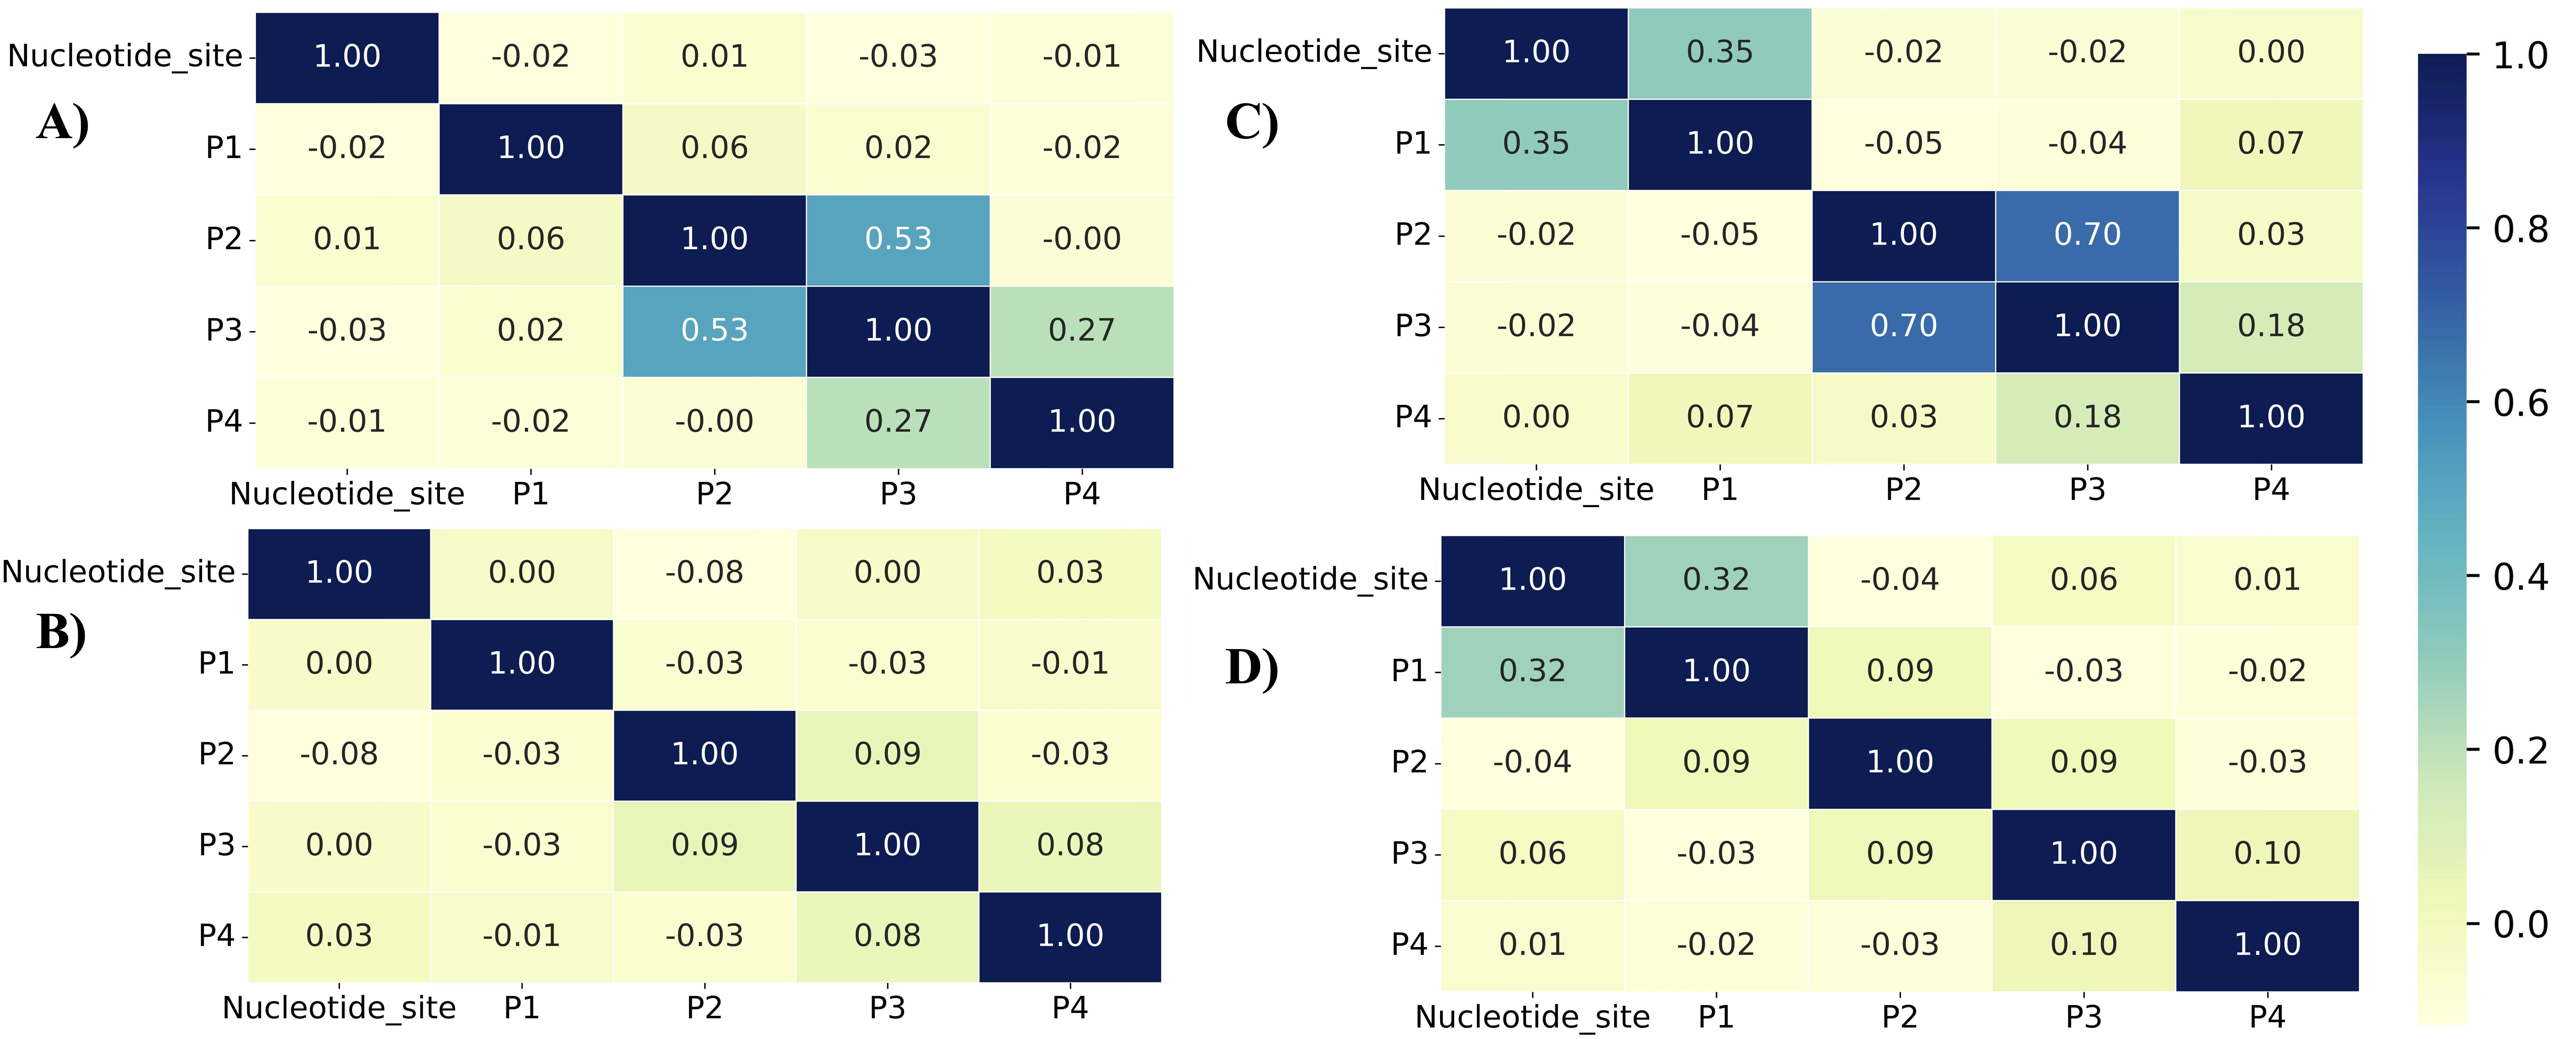
\includegraphics[width=1\textwidth]{Figcorr_nucleotide.jpg}
    \caption{Pearson Correlation for the volume fluctuations among different pockets and the effect of nucleotide binding. \textbf{A)} GDP-bound Rac1; \textbf{B)} GTP-bound Rac1; \textbf{C)} Nucleotide-free state created by deleting GDP from Rac1; \textbf{D)} Nucleotide-free state created by deleting GTP from Rac1.} 
    \label{fig:SI_CORRNUC}
\end{figure}

\begin{figure}[ht!]
    \centering
    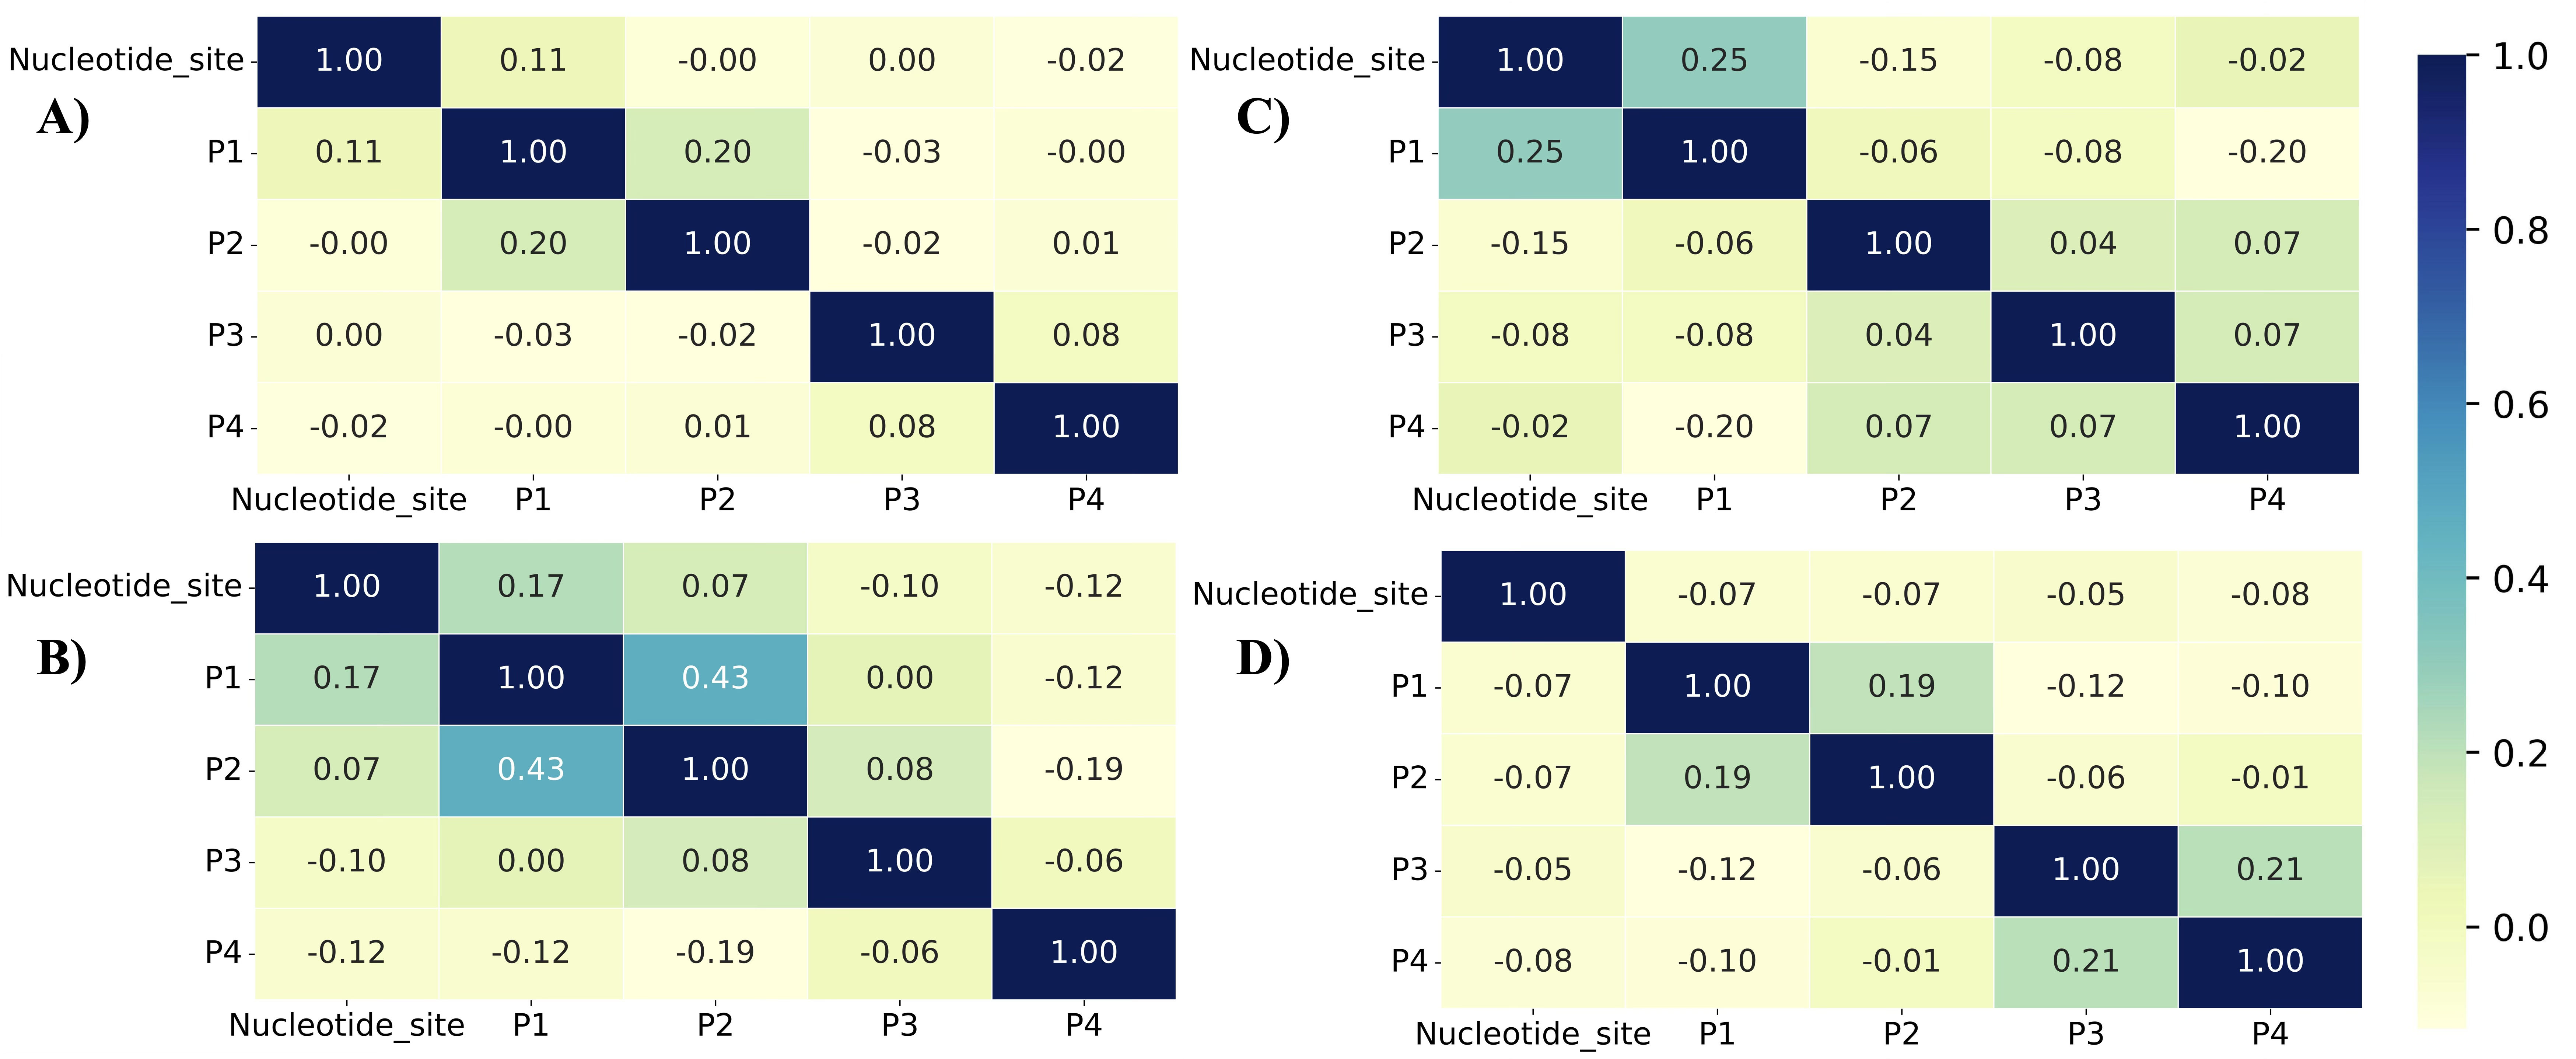
\includegraphics[width=1\textwidth]{Figcorr_gef.jpg}
    \caption{Pearson Correlation for the volume fluctuations among different pockets and the effect of GEF binding. \textbf{A)} PREX1-bound Rac1; \textbf{B)} TIAM1-bound Rac1; \textbf{C)}  VAV1-bound Rac1; \textbf{D)} DOCK2-bound Rac1. Rac1 in all GEF-bound systems is in the nucleotide-free state.} 
    \label{fig:SI_CORRGEF}
\end{figure}


\begin{table}
  \caption{Rac1 residues lining Site P1 with residuewise energy contribution to GEF binding}
  \label{tbl:SI_SiteP1}
  \begin{tabular}{c c c c c c}
    \hline
   \textbf{Residue} & \textbf{PREX1} & \textbf{TIAM1} & \textbf{VAV1} & \textbf{DOCK1} & \textbf{Comment} \\
    \hline
   T17 &  Y & Z & X1 & Y1 \\
   L20 &  Y & Z & X1 & Y1 \\
   T35 &  Y & Z & X1 & Y1 \\
   V36 &  Y & Z & X1 & Y1 \\
   F37 &  Y & Z & X1 & Y1 \\
   D38 &  Y & Z & X1 & Y1 \\
   N39 &  Y & Z & X1 & Y1 \\
   L55 &  Y & Z & X1 & Y1 \\
   W56 &  Y & Z & X1 & Y1 \\
   D57 &  Y & Z & X1 & Y1 \\
   T58 &  Y & Z & X1 & Y1 \\
   A59 &  Y & Z & X1 & Y1 \\
   G60 &  Y & Z & X1 & Y1 \\
   Q61 &  Y & Z & X1 & Y1 \\
   S71 &  Y & Z & X1 & Y1 \\
    \hline
  \end{tabular}
\end{table}

\begin{table}
  \caption{Rac1 residues lining Site P2 with residuewise energy contribution to GEF binding}
  \label{tbl:SI_SiteP2}
  \begin{tabular}{c c c c c c}
    \hline
   \textbf{Residue} & \textbf{PREX1} & \textbf{TIAM1} & \textbf{VAV1} & \textbf{DOCK1} & \textbf{Comment} \\
    \hline
   T17 &  Y & Z & X1 & Y1 \\
   L20 &  Y & Z & X1 & Y1 \\
   T35 &  Y & Z & X1 & Y1 \\
   V36 &  Y & Z & X1 & Y1 \\
   F37 &  Y & Z & X1 & Y1 \\
   D38 &  Y & Z & X1 & Y1 \\
   N39 &  Y & Z & X1 & Y1 \\
   L55 &  Y & Z & X1 & Y1 \\
   W56 &  Y & Z & X1 & Y1 \\
   D57 &  Y & Z & X1 & Y1 \\
   T58 &  Y & Z & X1 & Y1 \\
   A59 &  Y & Z & X1 & Y1 \\
   G60 &  Y & Z & X1 & Y1 \\
   Q61 &  Y & Z & X1 & Y1 \\
   S71 &  Y & Z & X1 & Y1 \\
    \hline
  \end{tabular}
\end{table}


\begin{table}
  \caption{Rac1 residues lining Site P3 with residuewise energy contribution to GEF binding}
  \label{tbl:SI_SiteP3}
  \begin{tabular}{c c c c c c}
    \hline
   \textbf{Residue} & \textbf{PREX1} & \textbf{TIAM1} & \textbf{VAV1} & \textbf{DOCK1} & \textbf{Comment} \\
    \hline
   T17 &  Y & Z & X1 & Y1 \\
   L20 &  Y & Z & X1 & Y1 \\
   T35 &  Y & Z & X1 & Y1 \\
   V36 &  Y & Z & X1 & Y1 \\
   F37 &  Y & Z & X1 & Y1 \\
   D38 &  Y & Z & X1 & Y1 \\
   N39 &  Y & Z & X1 & Y1 \\
   L55 &  Y & Z & X1 & Y1 \\
   W56 &  Y & Z & X1 & Y1 \\
   D57 &  Y & Z & X1 & Y1 \\
   T58 &  Y & Z & X1 & Y1 \\
   A59 &  Y & Z & X1 & Y1 \\
   G60 &  Y & Z & X1 & Y1 \\
   Q61 &  Y & Z & X1 & Y1 \\
   S71 &  Y & Z & X1 & Y1 \\
    \hline
  \end{tabular}
\end{table}


\begin{table}
  \caption{Rac1 residues lining Site P4 with residuewise energy contribution to GEF binding}
  \label{tbl:SI_SiteP4}
  \begin{tabular}{c c c c c c}
    \hline
   \textbf{Residue} & \textbf{PREX1} & \textbf{TIAM1} & \textbf{VAV1} & \textbf{DOCK1} & \textbf{Comment} \\
    \hline
   T17 &  Y & Z & X1 & Y1 \\
   L20 &  Y & Z & X1 & Y1 \\
   T35 &  Y & Z & X1 & Y1 \\
   V36 &  Y & Z & X1 & Y1 \\
   F37 &  Y & Z & X1 & Y1 \\
   D38 &  Y & Z & X1 & Y1 \\
   N39 &  Y & Z & X1 & Y1 \\
   L55 &  Y & Z & X1 & Y1 \\
   W56 &  Y & Z & X1 & Y1 \\
   D57 &  Y & Z & X1 & Y1 \\
   T58 &  Y & Z & X1 & Y1 \\
   A59 &  Y & Z & X1 & Y1 \\
   G60 &  Y & Z & X1 & Y1 \\
   Q61 &  Y & Z & X1 & Y1 \\
   S71 &  Y & Z & X1 & Y1 \\
    \hline
  \end{tabular}
\end{table}

\end{document}